\documentclass[ansiapaper]{report}
\usepackage[utf8]{inputenc}
\usepackage[english]{babel}
\usepackage[T1]{fontenc}
\usepackage{amsmath}
\usepackage{amsfonts}
\usepackage{amssymb}
\usepackage{makeidx}
\usepackage{graphicx}
\usepackage{float}
\usepackage{lmodern}
\usepackage[dvipsnames]{xcolor}
\usepackage{tikz}
\usetikzlibrary{intersections}
\usepackage{pgfplots}
\usetikzlibrary{calc}
\usepackage[ansiapaper]{geometry}
\geometry{hmargin=2cm,vmargin=2cm}
\usepackage{fancybox}
\usepackage{mathtools}
\usepackage{enumitem}
\usepackage{tcolorbox}
\usepackage{colortbl}
\usepackage{fancybox}
\tcbuselibrary{most}
\usepackage{pifont}
\usepackage[skip = 5pt, font = {footnotesize}, labelfont = sl]{caption}
\usepackage{subcaption}
\usepackage{eso-pic}
\usepackage{nicematrix}
\usepackage{multicol}
\usepackage{booktabs}
\usepackage{svg}
\usepackage{derivative}
\usepackage{wrapfig}
\usepackage{stmaryrd}
\usepackage{yfonts}
\usepackage{array}
\usepackage{csquotes}
\usepackage[style=phys , backend=biber]{biblatex}
\addbibresource{bibliography.bib}
\author{Andrea}
\setlength{\columnsep}{.5cm}
\usepackage[explicit]{titlesec}
\usepackage{lipsum}
\usepackage{indentfirst}
\usepackage{tabularx}
\usepackage{amsmath}
\usepackage{fancyhdr}
\usepackage{etoolbox}
\usepackage[export]{adjustbox}
\usepackage{fourier-orns}
\usepackage{lettrine}
\usepackage{physics}
\usepackage{hyperref}
\usepackage[capitalise]{cleveref}
\usepackage[titletoc]{appendix}
\usepackage{adforn}
\usepackage{cmbright}
\usepackage{wrapfig}
\usepackage{ulem}  % For paragraph underline
\definecolor{MyRed}{RGB}{197,112,93}
\definecolor{MySand}{RGB}{208,184,168}
\definecolor{MyWhite}{RGB}{248, 237, 227}
 %% Option 'familydefault' only if the base font of the document is to be sans serif
% use Roman numerals for sections
% \renewcommand\familydefault{\rmdefault}
\renewcommand{\thesection}{\Roman{section}}

% use Arabic numerals for subsections
\renewcommand{\thesubsection}{\Alph{subsection}}

% use letters for subsubsections with a parenthesis
\renewcommand{\thesubsubsection}{\alph{subsubsection})}

% put a period and space after numbers
\titlelabel{\thetitle\thickspace}

% % Make section titles centered and bold
\titleformat{\section}[block]
  {\MakeUppercase\normalsize\sffamily\bfseries}
  {\thesection .}{.3em}
  {\color{black}#1}

  \titleformat{\subsection}[block]
  {\centering\small\sffamily\bfseries}
  {\thesubsection .}{.3em}
  {\color{black}#1}

  \titleformat{\subsubsection}[block]
  {\small\sffamily\bfseries}
  {\thesubsubsection }{.3em}
  {\color{black}#1}
% \titleformat*{\subsection}{\bfseries}

\titleformat{\paragraph}[hang]
{\small\sffamily\slshape}
{\theparagraph}{.3em}
{\color{MyRed}#1}


\titleclass{\chapter}{straight}
\titleformat{\chapter}[block]
{\color{white}\large\sffamily\bfseries}
{}
{0em}
{\colorbox{MyRed}{\parbox{\dimexpr\linewidth-2\fboxsep\relax}{\centering \space#1}}}
[]
\titlespacing{\chapter}{0pt}{5pt}{5pt}
\titlespacing{\section}{0pt}{*3}{*3}
\titlespacing{\subsection}{0pt}{*1.5}{*1.5}
\titlespacing{\subsubsection}{0pt}{*1.5}{*1.5}


\hypersetup{
    colorlinks=false,
    linkbordercolor = {white},
    menubordercolor = {white},
    citebordercolor = {black},
    urlbordercolor = {black},
}
\captionsetup{singlelinecheck=off, box=colorbox,boxcolor=MyRed!20, labelsep=endash}

\pgfmathdeclarefunction{gauss}{2}{%
  \pgfmathparse{1/(#2*sqrt(2*pi))*exp(-((x-#1)^2)/(2*#2^2))}%
}
\usetikzlibrary{decorations.markings}
% \renewcommand{\headrule}{%
% \vspace{6pt}\hrulefill
% \raisebox{0pt}{\quad\adforn{64} \adforn{8} \adforn{36}\quad}\hrulefill}
% Page style setup
\pagestyle{fancy}
\fancyhf{} % Clear all header and footer fields

% Set the header height
\setlength{\headheight}{1cm}

% Custom header setup
\fancyhead[L]{%
    \begin{tikzpicture}[overlay, remember picture]
        \node[anchor=north west, xscale=1, yscale=1, minimum width=.7\paperwidth, minimum height=\headheight, fill=MyRed, text=white, inner sep=0pt, outer sep=0pt, line width=0pt] at ([yshift=-0.7cm]current page.north west) {\parbox[c][\headheight]{.7\paperwidth}{\sffamily{\hskip2cm \textbf{\leftmark \hfill \small{Master SdM}\hspace{.5cm} }}}};
        \node[anchor=north east, xscale=1, yscale=1, minimum width=.2\paperwidth, minimum height=\headheight, fill=white, text=MyRed, inner sep=0.5pt, outer sep=0pt, line width=0pt] at ([yshift=-0.7cm, xshift=-1cm]current page.north east) {\parbox[c][\headheight]{.3\textwidth}{\centering\sffamily{\textbf{\small{ENS | ENSL}}}}};
        \draw[MyRed, line width=0.3mm]
        ([yshift=-0.7cm, xshift=-1.75cm]current page.north east)
        rectangle ([xshift=-\paperwidth*0.3+.5cm, yshift=-1.65\headheight-0.3mm]current page.north east);
        \node[fill=MyRed, inner sep=0pt, line width=0pt, minimum width=.12\paperwidth, minimum height=\headheight] (github) at ([yshift=-1.2cm, xshift=.1cm]current page.north east)  {
            \begingroup
            \hypersetup{pdfborder={0 0 0}}
            \hspace{-1.5cm}\href{https://github.com/Chatr0uge/Internship_SPC}{
\includegraphics[height=1cm]{./figures/github.png}}
            \endgroup
    };
    \end{tikzpicture}
}

% Remove the default header rule (optional)
\renewcommand{\headrulewidth}{0pt}
\newcommand*{\defeq}{\stackrel{\text{def}}{=}}

\rfoot{Andrea Combette}
\fancyfoot[C]{\thepage}

\newlength{\tabcont}


\setcounter{tocdepth}{2}
\setcounter{secnumdepth}{4}

\begin{document}

% Custom header setup with tabular



\fontsize{9}{10}\selectfont%

\renewcommand{\contentsname}{Contents} % Rename ToC title


\vskip6pt
\begin{center}
  \noindent \sffamily{\textbf{\Large Lectures notes on Advanced Computational Statistical Physics}}
\end{center}
\vskip9pt

\begin{multicols}{3}

  \renewcommand{\baselinestretch}{1.1}\normalsize % Adjust spacing of ToC
  {\footnotesize \sffamily \tableofcontents} % Set font size for ToC



  \renewcommand{\baselinestretch}{1.0}\normalsize

  \fontsize{9}{10}\selectfont
  \chapter{Introduction}
  In the 19th century, classical mechanics, rooted in Newton’s laws, dominated physics. Pierre-Simon Laplace famously articulated the deterministic worldview: given the initial conditions of a system, its future could be perfectly predicted through precise mathematical equations. This perspective treated the universe like a clockwork machine, where every event followed from the initial state.

  However, as the study of thermodynamics and many-particle systems advanced, the limits of this purely deterministic approach became clear. Statistical physics emerged to address these complexities, particularly through the work of James Clerk Maxwell and Ludwig Boltzmann. Their pioneering contributions, such as Maxwell's velocity distribution in gases and Boltzmann's statistical interpretation of entropy, introduced probabilistic methods to understand the behavior of large ensembles of particles.

  In this new framework, the precise motion of individual particles became less important; instead, statistical averages and distributions described macroscopic properties like temperature and pressure. While Laplace envisioned a universe governed by strict determinism, statistical physics embraced the unpredictability inherent in large systems, marking a profound shift in understanding.

  This shift continued to resonate into the 20th century, influencing the work of physicists like Philip W. Anderson. Anderson famously argued that "more is different," suggesting that the behavior of complex systems cannot be fully understood by analyzing individual components alone. This echoes the insights of 19th-century statistical physics, where collective behavior emerged from many interacting parts, challenging the reductionist views of classical mechanics.

  In summary, while classical mechanics remained essential for describing deterministic systems, the development of statistical physics in the 19th century introduced a probabilistic approach that transformed our understanding of many-body systems and laid the groundwork for modern physics.

  \section{Computational Statistical Physics}

  Computational methods allow us to simulate these complex systems directly, providing detailed insights into their behavior. Using modern computing power, scientists can model the interactions of millions, or even billions, of particles, making it possible to observe emergent phenomena such as phase transitions, critical behavior, and chaotic dynamics. This computational approach helps us overcome the "many-body" problem, where the sheer number of interactions in a system defies exact solutions.

  One reason computational statistical physics is so powerful is that it can handle systems that are analytically intractable. For instance, systems with strong correlations between particles or those far from equilibrium, which are difficult to study using traditional methods, can be simulated using Monte Carlo techniques, molecular dynamics, and other algorithms.

  Additionally, computational approaches enable the study of phenomena at different scales—from the atomic scale, where quantum effects dominate, to macroscopic scales governed by classical statistical physics. This versatility allows for a deeper understanding of both microscopic mechanisms and their macroscopic consequences, bridging the gap between theoretical models and real-world systems.

  In essence, computational statistical physics allows us to explore systems that are too complex for exact solutions, providing a practical and powerful way to study emergent behavior, phase transitions, and non-equilibrium systems. By leveraging the power of computers (which is increasing exponentially since the second half of the 19th century \cref{fig:supercomputer_flops}), it opens up new frontiers for understanding the vast complexity of the physical world, which neither classical mechanics nor early analytical statistical methods could fully address.

  \begin{figure}[H]
    \centering
    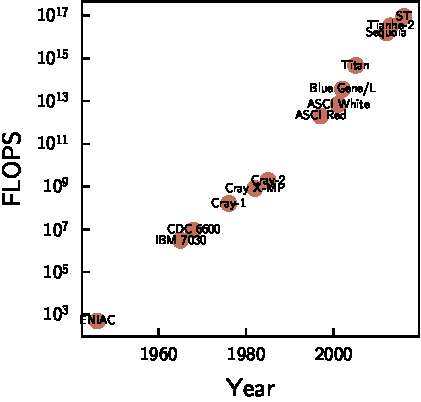
\includegraphics[width=1\linewidth]{./figures/supercomputer_flops.pdf}
    \caption{Number of Floating points operations evolution for the biggest supercomputer \label{fig:supercomputer_flops}}
  \end{figure}

  \section{Invariant Measures and Ergodicity}

  In statistical physics, the concept of an invariant measure plays a crucial role in understanding the long-term behavior of dynamical systems, and the symetry of the system (Noether's theorem). One of the main goals of computational statistical physics is to find algorithms preserving the invariant measure of the systems we are studying. For example we will see that the Euler algorithm is not a good choice for simulating Hamiltonian systems, as it does not conserve the energy of the system, as opposed to the Verlet algorithm, which is based on clever considerations of the symplectic\footnote{Refers to the Hamiltonian Formulation of classical mechanics} structure of the phase space.

  Ergodicity is another important concept in statistical physics, which ensures that the system explores the entire phase space in the long run. Which results in one of the most important hypothesis in computational statistical physics, the ergodic hypothesis, which states that the time average of a system is equal to its ensemble average (limit cases CITE).

  \chapter{Molecular Dynamics}
  \section{Hamiltonian Dynamics}
  \subsection{Hamiltonian Formalism}

  The Legendre transformation of the Lagrangian allows us to define the Hamiltonian of a system, which is a function of the generalized coordinates $q_i$ and the generalized momenta $p_i$ of the system (see CITE). The Hamiltonian is defined as :
  $$ H \defeq \frac{\textbf{p} ^T \textbf{M} ^{-1} \textbf{p}  }{2} + U(q)$$
  with $U(q)$ the potential energy of the system and $\textbf{M}$ the mass matrix of the system. The equations of motions can then be written using the Euler-Lagrange equations :
  $$
    \begin{cases}
      \dot{q} = \frac{\partial H}{\partial p} \\
      \dot{p} = -\frac{\partial H}{\partial q}
    \end{cases}
  $$

  This can be written in a more compact matrix form :

  $$ \begin{pmatrix}
      \dot{\textbf{q} } \\
      \dot{\textbf{p} }
    \end{pmatrix} = \textbf{J} \nabla H(\textbf{p} ,\textbf{q} )
  $$
  with $$\textbf{J} = \begin{pmatrix}
      0          & \textbf{I} \\
      \textbf{I} & 0
    \end{pmatrix} $$
  These type of non linear equations can only be locally, but since the systems are Hamiltonian we can unearth the global existence and uniqueness of the solutions. Indeed we just need to show that using the energy constraints of the system the solutions are bounded for all time. For the impulsion this is trivial considering a potential global minimum :

  $$ \frac{\textbf{p}^T \textbf{M} ^{-1} \textbf{p} }{2} \leq E_0 - U_{min}$$

  for the position we just need an assumption on the level sets of the potential energy. $$ \Sigma_{\alpha} = {\textbf{q}|U(\textbf{q} = \alpha) }$$
  If these lebel are bounded then the solutions are bounded for all time. This is not the case for all potentials, this is why for solving this kind of equations we will add sometimes confining potentials to the system.
  \subsection{Map Flow}

  Since the Hamiltonian equations are solvable, it seems natural to define a map flow $\mathcal{F}$ such that for an initial condition $z_0$ and a considered point $z_t$ we have :
  $$\textbf{z} _t = \mathcal{F}_t(\textbf{z}_0)$$
  This flow map is obviously invertible and Hamiltonian conservative. The key of numerical integration is then to approximate the true flow map of the system by the numerical flow map $\mathcal{T}$ such that the physical properties of the system are conserved over time.

  Considering the linear system for the differentiation :

  \begin{equation}
    \label{eq:linear_system}
    \dv{\textbf{z}}{t} = f(\textbf{z} ) = A\textbf{z}
  \end{equation}

  One way to solve this equation is to use the matrix exponential :

  $$\textbf{z}_t = \exp(At)\textbf{z}_0$$

  Then it appears that the flow map is given by :
  \begin{equation}
    \label{eq:flow_map}
    \mathcal{F}_t(\textbf{z} ) = \exp(tA)\textbf{z}
  \end{equation}

  \subsection{Sympletic Form}

  \subsubsection{Volume Preservation}
  One of the most important properties of the flow map is the preservation of the volume in the phase space. Indeed,for a Hamiltonian system we have thanks to Liouville's theorem the volume of a given sets of solution governed by \cref{eq:linear_system} is preserved over time if $$ \nabla \cdot f = 0 \, .$$

  It is easy to show that for a Hamiltonian system : $$\nabla \cdot f = \nabla \cdot \begin{pmatrix}
      0          & \textbf{I} \\
      \textbf{I} & 0
    \end{pmatrix} \nabla H = 0$$
  Due to the $\mathcal{C}^2$ property of the Hamiltonian. The main consequence of this property is that the flow map is volume preserving, which has to be a important property of the integration algorithm to approximate the flow map.

  Volume preservation is a key prroperty since it ensures that the numerical integration keeps the hamiltonian structure of the system, following the loiouville theorem i.e the conservation of the phase space volume along particles trajectories in the phase space.

  \begin{figure}[H]
    \def\svgwidth{\linewidth}
    \input{./figures/Phi_space_volume.pdf_tex}
    \caption{Volume conservation for the true Hamiltonian in black and the approximated Hamiltonian in red}
    \vspace{0.15cm}
  \end{figure}

  \subsubsection{Sympletic Property}
  The sympletic property of the flow map is another important property of the Hamiltonian system. Indeed, the sympletic property of the flow map is defined as :
  $$ \mathcal{F}_t^T J \mathcal{F}_t = J$$
  With $J = \begin{pmatrix}
      0           & \textbf{I} \\
      -\textbf{I} & 0
    \end{pmatrix}$ the sympletic matrix. This property leeads to the conservation of the volume of the phase space, indeed we have  for the jacobian associated with the map : $\lvert \mathcal{F'}_t\rvert^2 = 1 $.

  One intersting point of symplectic maps is that they form a group (they preserved the composition) which can be used to build other more complex symplectic maps. For example to increase the order of sympletic integrators $\mathcal{G}_h$  approximating the flow map $\mathcal{F}_h$, we can also split wut Hamiltonian just dependant of the impulsion or the position. This is called the splitting method, which is based on the Trotter expansion of the flow map (Find sympletic form of splitted hamiltonian).

  \subsection{Error Analysis for Hamiltonian splitting}


  \subsubsection{Lie Derivatives and Poisson Brackets}

  \paragraph*{Lie Derivatives}

  In the case of a non-Linear Hamiltonian system, the flow map can be approximated by the Lie derivative of the Hamiltonian, we would like to find again the conveninant results :

  $$ \mathcal{F}_t = \exp(tA)\textbf{z}$$

  Let's consider a functionnal $\Phi$ f the phase space, the Lie derivative of $\Phi$ is defined as :

  $$ \mathcal{L}_f \Phi = \nabla \Phi \cdot A$$

  This is a generalization of the directional derivative to the phase space. Expanding the $\Phi$ map in a Taylor series we have :

  \begin{align*}
    \\ \Phi(\textbf{z}(t)) &= \sum_i \frac{t^i}{i!}(\mathcal{L}_f^i \Phi)( \Phi(\textbf{0} ))
    \\ &= \exp(t\mathcal{L}_f)(\Phi(\textbf{0}) )
  \end{align*}

  Applying this to the identity gives us the following map :

  $$\mathcal{F}_t(\textbf{z} ) = \exp(t\mathcal{L}_f)(\textbf{z})$$

  As we wanted.

  \paragraph*{Poisson Brackets}

  A common notation introduced in Hamiltonian mechanics is the Poisson bracket, which is defined as :

  \begin{align*}
    \\ \{g_1, g_2 \} &= \sum_{i = 1}^N (\pdv{g_1}{q_i}\pdv{g_2}{p_i} - \pdv{g_2}{q_i}\pdv{g_1}{p_i})
    \\ &= \nabla g_1^T \textbf{J} \nabla g_2
  \end{align*}

  Considering a smoooth scalar value function $F$ of the phase space, we can show that the Lie derivative of $F$ is given by the Poisson bracket of $F$ and the Hamiltonian :

  $$ \mathcal{L}_{\textbf{J} \nabla H} F = \mathcal{L}_H F = \{F, H\}$$

  Poisson brackets can be related to the Lie derivating noticing that for every real valued function $f$: $$[\mathcal{L}_{H_1}, \mathcal{L}_{H_2}]f = \mathcal{L}_{\{H_1, H_2\}}f$$

  \subsubsection{Error Analysis for non Commuting Hamiltonian}
  The main idea behinds this study is to consider integration method as a splitting of the Hamiltonian into several parts oftenly independant of one of the two system of coordinates $(\textbf{q}, \textbf{p})$, as we will see further. The poisson brackets are linear with respect to the Hamiltonian, which allows us to write the following considering $H = H_1 + H_2$,

  $$\mathcal{L}_H = \mathcal{L}_{H_1} + \mathcal{L}_{H_2}$$

  The flow map of the system is then defined as : $\mathcal{F}_t(\textbf{z}) = e^{t()\mathcal{L}_{H_1} + \mathcal{L}_{H_2})}\textbf{z}  $

  The splitting method has the following flow map : $$\mathcal{G}_th= e^{h\mathcal{L}_{H_1}}e^{h\mathcal{L}_{H_2}}$$ Which is not the same as the true flow map. To evaluate the error done considering the splitted Hamiltonian, we can use the Baker-Campbell-Hausdorff formula [CITE] and the correspondance between the Lie derivative and the Poisson bracket unearthing :

  $$ e^{h\mathcal{L}_{H_1}}e^{h\mathcal{L}_{H_2}} = e^{ h \mathcal{L}_{\tilde{H}_h}}$$

  With $\tilde{H}_h$ the \textit{shadow Hamiltonian} :

  \begin{multline*}
    \tilde{H}_h = H_1 + H_2 + \frac{h}{2}\{H_1 , H_2 \} + \\
    \frac{h^2}{12}(\{H_1 \{H_1 , H_2\} \} - \{H_2 \{H_1 , H_2 \} \}) \dots
  \end{multline*}


  From this we can easily understand that as long as the two splitted Hamiltonian do not commute, we have at least an linear error (on example is the sympletic Euler Method). One way to do that, is to find a split with commutating hamiltonian, or to split $H$ into three hamiltonian such that that the linear term vanishes (such as the Velvet velovity \& position method). The main indea behind this  development was to show that the flow map $\mathcal{F}_t$ we approximate using the other $\mathcal{G}_t$ stands in the splitting method for an exact solution to a other (but similar) hamiltonian system.

  To put in a nutshell the splitting method allows us to build sympletic integrator using Hamiltonian transformations. Not all intersteing integrators have sympletic structures, but they should all conserve volume in the phase space.




  \section{Time Integration}

  Here we will restrict our study to linear system. To perform time integration, we discretize time into small intervals $\delta t$ . At each time step $t_{n+1}=n \delta t$, we approximate the change in the system using matrix iteration.
  $$ \begin{pmatrix}
      x(n\delta t) \\
      y(n\delta t)
    \end{pmatrix} = \mathcal{T}^n(\delta t) \begin{pmatrix}
      x(0) \\
      y(0)
    \end{pmatrix}$$

  The goal is then to find the correct matrix such that iterating over time will not change the invariance of the system. To fitt he previous notation the flow map can be defined as :
  $$\mathcal{F}_{\delta t}(\textbf{z} ) = T(\delta t)\textbf{z} $$

  \subsection{Application to the Harmonic Oscillator}

  \subsubsection{Exact Propagator}

  For the harmonic oscillator, the time evolution is well known which is useful to test the time integration algorithms. Indeed, we got :

  $$ \begin{pmatrix}
      x(\delta t) \\
      y(\delta  t)
    \end{pmatrix} = \mathcal{T}(\delta t) \begin{pmatrix}
      x(0) \\
      y(0)
    \end{pmatrix}$$
  With $$\mathcal{T}(\delta t) =  \left(\begin{array}{cc}
        \cos(wt)    & \frac{1}{w}\sin(wt) \\
        \-w\sin(wt) & \cos(wt)
      \end{array}\right)$$

  In the next analysis we will use a dimensionless time $\tau = \omega t$,  a dimensionless position $\xi = \sqrt{\frac{k}{k_BT}x}$ and a dimensionless impulsion $\Pi = \sqrt{\frac{1}{mk_bT}}p$ , which leads to the following time Propagator :
  \begin{align*}
    \\ \mathcal{L}_{\delta \tau} = \mathcal{T}(\delta \tau) &=  \left(\begin{array}{cc}
        \cos(\delta \tau)   & \sin(\delta \tau) \\
        - \sin(\delta \tau) & \cos(\delta \tau)
      \end{array}
    \right)
    \\ &=  \exp(\textbf{J}h)
  \end{align*}

  Here we related as did previously the flow map to the derivative operation for our system.
  For the Hamiltonian we find :

  $$ H = \frac{\mathcal{H}}{k_BT} = \frac{1}{2}(\Pi^2 + \xi^2)$$. Then let's consider a microstate of the system $\ket{\tau} = \begin{pmatrix}
      \xi(\tau) \\
      \Pi(\tau)
    \end{pmatrix}$
  The time evolution of the system is given by the following equation :
  $$ \ket{\tau + \delta \tau} = \mathcal{T}(\delta \tau) \ket{\tau}$$
  With the unitary propagation matrix $$\mathcal{T}(\delta \tau) = \begin{pmatrix}
      \cos(\delta \tau)         & \frac{1}{\omega}\sin(\delta \tau) \\
      -\omega \sin(\delta \tau) & \cos(\delta \tau)
    \end{pmatrix}$$
  Solvning the characteristic equation $\lVert \mathcal{T} - \lambda I\rvert = 0$, we unearth the eigenvalues.
  $$ \lambda_\pm = \exp(\pm i \delta \tau), $$

  Considering the two \textbf{orthogonal}  eigenvectors $\ket{\pm}$, we easily show that :
  \begin{align*}
    \ket{n \delta t} & = \mathcal{T}(\delta t)^n \ket{0}                   \\
                     & = a_+ \lambda_+^n \ket{+} + a_- \lambda_-^n \ket{-} \\
  \end{align*}

  Considering the initial decomposition $$ \ket{0} = a_+ \ket{+} + a_- \ket{-}$$

  Then we can easily show that :

  \begin{align*}
    \\ \frac{E}{k_bT} &= \frac{1}{2}\braket{n \delta \tau}{n \delta \tau}
    \\ &=\frac{1}{2}\left(\lvert a_+ \rvert^2 \lvert a-+ \rvert^2 \right)\mathcal{T}(\delta t)^n
    \\ &= \frac{1}{2} \braket{0}{0}
  \end{align*}

  Which shows that the energy is conserved over time. We can also show an interesting result about the conserved quantities :

  \begin{align*}
    \\ \expval{A}{0} &=\expval{A}{\tau}
    \\  & \Rightarrow A \equiv \mathcal{T}^\dagger A \mathcal{T}
    \\ & \Rightarrow A \propto H
  \end{align*}

  \subsubsection{Euler Algorithm \& Propagator}

  The Euler algorithm is the simplest algorithm to perform time integration, based on the first order approximation in Taylor expansion. We obtain the following propagation matrix :

  $$ \mathcal{T}(\delta \tau) =
    \begin{pmatrix}
      1                     & \delta \tau \\
      -\omega^2 \delta \tau & 1
    \end{pmatrix}
  $$

  Which is not unitary, and thus does not conserve the energy of the system. We can show that the energy of the system is not conserved over time, though the same reasoning as before. The two eigenvalues of the matrix are :

  $$ \lambda_\pm = 1 \pm i \delta \tau$$

  Which leads to divergence of the energy with the following expression :

  \begin{align*}
    H & = \frac{1}{2}\braket{0}{0}(1 + \delta \tau^2)^n          \\
      & = \frac{1}{2}\braket{0}{0}\exp(n \ln(1 + \delta \tau^2))
    \\
  \end{align*}

  This divergence of the system can be seen in the following figure \cref{fig:HarmonicOscillator}

  \subsubsection{Verlet Algorithm \& Propagator}

  The Verlet algorithm is a second-order algorithm, which is based on the symplectic structure of the phase space and directly derived from the Trotter expansion as we will see after. The scheme is given by the following :
  $$
    \begin{cases}
      x(t + \delta t) = x(t) + \delta t v(t) + \frac{\delta t^2}{2} a(t) \\
      v(t + \delta t) = v(t) + \frac{\delta t}{2} (a(t) + a(t + \delta t))
    \end{cases}
  $$
  The Propagator in the dimensionless space is then given by the following matrix :

  $$ \mathcal{T}(\delta \tau) = \begin{pmatrix}
      1 - \frac{\delta \tau^2}{2}                             & \delta \tau                 \\
      -\delta \tau \left(1 - \frac{1}{4} \delta \tau^2\right) & 1 - \frac{\delta \tau^2}{2}
    \end{pmatrix}
  $$

  Here we find an unitary matrix, which conserves the pseudo energy of the system over time. Indeed using this scheme the eigenspaces are not orthogonal anymore, the true energy is then not conserved however we can still study the conserved quantities and show that :

  \begin{align*}
    \expval{A}{0} & = \expval{A}{\tau}
    \\ & \Rightarrow A \equiv \mathcal{T}^\dagger A \mathcal{T}
    \\ & \Rightarrow A \propto \begin{pmatrix}
      1 & 0                                 \\
      0 & \frac{1}{(1 - \delta \tau^2/2)^2}
    \end{pmatrix}\underset{\delta \tau \rightarrow 0}{\longrightarrow} \propto H
  \end{align*}


  \begin{figure}[H]
    \centering
    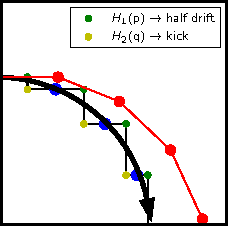
\includegraphics[width=1\linewidth]{./figures/Velvet_euler.pdf}
    \caption{\label{fig:sample} Phase space of the Harmonic Oscillator for different time integration algorithms, we clearly see the divergence of the energy for the Euler algorithm and the notable conservation of the energy for the Verlet algorithm.}
  \end{figure}

  \begin{figure}[H]
    \centering
    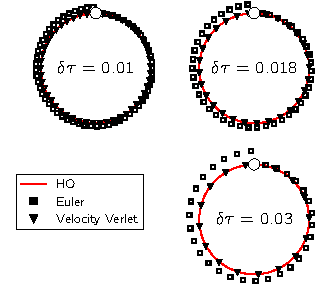
\includegraphics[width=1\linewidth]{./figures/HarmonicOscillator.pdf}
    \caption{\label{fig:sample} Phase space of the Harmonic Oscillator for different time integration algorithms, we clearly see the divergence of the energy for the Euler algorithm and the notable conservation of the energy for the Verlet algorithm.}
  \end{figure}

\end{multicols}

\end{document}
